\documentclass{standalone}
\usepackage{tikz}
\usepackage{ifthen}

\begin{document}
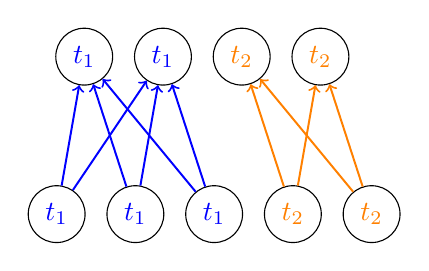
\begin{tikzpicture}
  % Bottom row
  % Nodes 1-2 are important for task t_1
  % Node 3-4 is important for task t_1
  %\node[circle, draw] (bottom\x) at (\x-0.35,0) {$\label$};
  %\node[circle, draw, text=blue] (bottom\x) at (\x-0.35,0) {$\label$};
  \foreach \x/\label in {1/t_1, 2/t_1, 3/t_1, 4/t_2, 5/t_2}
    \ifthenelse{\equal{\label}{t_1}}
        {\node[circle, draw, text=blue] (bottom\x) at (\x-0.35,0) {$\label$};}
        {\node[circle, draw, text=orange] (bottom\x) at (\x-0.35,0) {$\label$};};
  
  % Top row
  \foreach \x/\label in {1/t_1, 2/t_1, 3/t_2, 4/t_2}
    \ifthenelse{\equal{\label}{t_1}}
        {\node[circle, draw, text=blue] (top\x) at (\x,2) {$\label$};}
        {\node[circle, draw, text=orange] (top\x) at (\x,2) {$\label$};};
        
  % Arrows from bottom row t_1 to all top row 
  \foreach \x in {1,2,3}
    \foreach \y in {1,2}
      \draw[->, blue, line width=0.25mm] (bottom\x) -- (top\y);

  \foreach \x in {4,5}
    \foreach \y in {3,4}
      \draw[->, orange, line width=0.25mm] (bottom\x) -- (top\y);

  % \node[] at (-0.5, 2) {$\ell$};
  % \node[] at (-0.5, 0) {$\ell-1$};
      
\end{tikzpicture}
\end{document}